\documentclass[11pt]{article}
\usepackage{geometry}                % See geometry.pdf to learn the layout options. There are lots.
\geometry{letterpaper}                   % ... or a4paper or a5paper or ... 
%\geometry{landscape}                % Activate for for rotated page geometry
%\usepackage[parfill]{parskip}    % Activate to begin paragraphs with an empty line rather than an indent
\usepackage{graphicx}
\usepackage{amssymb}
\usepackage{epstopdf}
% Package for including code in the document
\usepackage{listings}

\usepackage{algorithm,algorithmic}
\DeclareGraphicsRule{.tif}{png}{.png}{`convert #1 `dirname #1`/`basename #1 .tif`.png}

\title{Expected Maximization as part of a Bayesian/Gaussian Framework}
\author{Dan Beatty}
%\date{}                                           % Activate to display a given date or no date

\begin{document}
\maketitle
%\section{}
%\subsection{}

\section{Overview of EM}
%Most texts on Expected Maximization (EM) claim that 
The goal of the EM algorithm is to determine a set of parameters that define a statistical model given a certain data set.   If the data set is incomplete, then is some representation of the complete data set.  If the data set can be represented by a set of statistical distributions,  then EM can be used to obtain the sufficient statistics of those distributions.  %The assumption in this algorithm is that the given data set is incomplete and is representative of a data set with more attributes than are present in the data set.  %Thus despite the number of samples, the missing attributes render the system underdetermined/
EM extends properties of maximum likelihood estimation methods by determining via iterative convergence the governing parameters of a particular data-set.   In particular,  uncorrupted cases may use sufficient statistics acquired via MLE,  \cite{duda-hart-stork}.  
%There were few points made in \cite{duda-hart-stork} claimed that EM was an extension of the maximum likelihood method as a method determining governing parameters for a given data set, with an assumed model, and given data set points.  
%\begin{itemize}
%	\item Uncorrupted cases could use $\hat{\vec{\theta}}$ acquired from MLE.
%	\item Iteratively converge on the likelihood for a given data set via Expectation Maximization or Baum-Welch
%	\item Features can be in terms of good features and bad features:  $D = \{ \vec{x_1} ,\ldots,\vec{x_n} \}$ or $D = D_g \cup D_b$.
%	\item 
%\end{itemize}
In general, the equation for the terminating condition of the EM algorithm \cite{duda-hart-stork} is stated in equation \ref{em_basis} .  The meaning of the terms in equation \ref{em_basis} are as follows:
%Also stated in most text, the general equation for the EM algorithm is defined in equation \ref{em_basis} where
\begin{itemize}
\item  $\mathbf{X}$ is the true data set, $\vec{x}$ is the true data set sample, 
 \item $\vec{\Theta}$ are the set of parameters for the statistic, and 
 \item $\vec{y}$ is the data sample in the given data set.
 \end{itemize}
\begin{equation}
\vec{\Theta}^* = \arg \max_{\Theta} \sum_{\vec{x}\in \mathcal{X}^n} E[ \ln p( \mathbf{x} | \vec{\theta} ,\vec{y}) ] \label{em_basis}
\end{equation}
Equation \ref{em_basis} may be refined into \ref{duda-hart-stork-EM} with the following notation obtained from \cite{duda-hart-stork}:
%The one presented in \cite{duda-hart-stork} is presented in equation \ref{duda-hart-stork-EM}.  The notation is defined as follows:
\begin{equation}
Q( \vec{\theta} ; \vec{\theta}^i) = E_{D_b} [ \ln p(D_g, D_b; \vec{\theta}) | D_g ; \vec{\theta}^i ] \label{duda-hart-stork-EM}
\end{equation}
\begin{itemize}
	\item $\vec{\theta}^i$ is the current (best) estimate for the full distribution;  
	\item $\vec{\theta}$ is a candidate vector for an improved estimate 
	\item $Q(\vec{\theta} ; \theta^i)$ is a function of $\vec{\theta}$ and $\vec{\theta}^i$
	\item $D_b$ is the actual data set.  
	\item $D_g$ is the unknown and uncorrupted data set.
	\item $E_{D_b} [ \ln p(D_g, D_b; \vec{\theta}) | D_g ; \vec{\theta}^i ] $ is the expected value over the missing features.  The expected value hinges on $\vec{\theta}^i$ which are the true parameters.
\end{itemize}
One of the goals is marginalize $D_b$ with respect to $\vec{\theta}^i$.  Another goal of the EM algorithm is select from the candidate $\vec{\theta}$ from a set of $\vec{\theta}$s, and iterate to a $\vec{\theta}^{i+1}$ which yields the greatest $Q(\vec{\theta} ; \vec{\theta}^i)$.  In order for EM to work the assumption of that $D_g$ is an independent and identically distributed (i.i.d) observations must hold. 
%	\item Samples are assumed identically independent distribution (iid).  





\subsection{Specification for Gaussian Case}
In the Gaussian case, each class has a proportion that defines how much its class contributes, a mean and covariance (denoted $\alpha, \vec{\mu}, \mathbf{\Sigma}$ respectively) .   If one acquires a sample as a initial set, the question is does an EM algorithm that will refine these sufficient statistics?   %One paper by Frank Dellaert shows an example of yes.  The Q function is presented as a matrix, which must be reduced to a form that allows the less than operator to be valid.  
In \cite{yamazaki98introduction}, there is an example using a matrix as the result of the expectation step.  From this expectation, the sufficient statistics for the next step is computed.   The expected equation is as in equation \ref{expectedMatrix} forms a matrix $\mathbf{A}$ called the expected matrix.
\begin{equation}
a_{ij}^{(k)}     = \frac {\alpha_j p(\vec{y}_i  ^{(k)}  | \vec{\mu_j} ^{(k)} , \Sigma_j ^{(k)}  )}{\sum_{j=1}^M \alpha_j p(\vec{y}_i  ^{(k)}  | \vec{\mu_j} ^{(k)} , \Sigma_j ^{(k)}  )} \label{expectedMatrix}
\end{equation}


The three sufficient statistics are computed in the maximization step.   It is computed by
\begin{eqnarray}
\vec{\mu} _j ^{(k+1)} = \frac{\sum_{i=1} ^N a_{ij}^{(p)} \vec{y}_i} {\sum_{i=1}^N a_{ij} } \\
\mathbf{\Sigma} _j ^{(k+1)} = \frac {\sum_{i=1}^N (\vec{y}_i \vec{\mu}_j ^{(p)} )^T(\vec{y}_i \vec{\mu}_j ^{(p)} ) } {\sum_{i=1}^N a^{(k)}_{ij}}  \\
\alpha _j ^ {(k+1)} = \frac{1}{N} \sum_{i=1}^N a^{(k)}_{ij}
\end{eqnarray}



The obvious question is what reduction on $\mathbf{A}$ is used to assess the convergence of the estimations.  %In this case, the determinant is used since it is always positive.    Another question is where is the proof that $|\mathbf{A}|$ is monotonic, in each iteration.  
\begin{equation}
Q ( \theta ^* ; \theta ) =\log (\prod_{i=1} ^N  a_{ii} )
\end{equation}


Another observation, it is clear that the initial guess can not be the zero matrix.  As such, the sufficient statistics would be rendered zero, and no convergence would occur.   Typically, the guesses are for $\mu$ to be scattered for each class, and for the expected matrix to be 
\[ 
\mathbf{A} = \frac{1}{N} \mathbf{I}.
\]

%\section{Implementation}
%This particular framework class Objective-C class includes the computation of the expected matrix ($\mathbf{A}$) in the the expected method.  Likewise, the sufficient statistics are computed in the maximization step.  One thing of note is that each step is stored in an NSMutableArray.  This is definitely not efficient memory wise, but it is simple to implement.  The samples are all row vectors held in a matrix.  

In the most basic notion, the EM Algorithm should be implemented as stated in its algorithm, Algorithm \ref{alg:expectation-maximization}.  Such an Objective C implementation is listed in \ref{lst_computeEM}.  Notice though the expected step and maximization step are separate methods, and may be considered private methods and overridden in each subclass.  In this case, they are publicly accessible although only the computeEM and probability classes need to be called to obtain the parameters.  


\begin{algorithm}
\caption{Expectation Maximization}
\label{alg:expectation-maximization}
\begin{algorithmic}
	\STATE initialize $\vec{\theta}^0$, $T$, and $i \leftarrow 0$
	\REPEAT
		\STATE $i \leftarrow i + 1$
		\STATE \textbf{E Step:} compute $Q(\vec{\theta} ; \vec{\theta}^i)$ 
		\STATE \textbf{M step:} $\theta ^{i+1} \rightarrow \arg \max _{\theta} Q(\vec{\theta} ; \vec{\theta} ^i)$ 
	\UNTIL {$Q(\vec{\theta}^{i+1} ; \vec{\theta}^i) - Q(\vec{\theta}^{i} ; \vec{\theta}^{i-1}) \le T$}
	\RETURN {$\hat{\vec{\theta}} \rightarrow \vec{\theta}^{i+1}$}
\end{algorithmic}
\end{algorithm}

\begin{lstlisting} [ language={[Objective] C} ,caption={Compute EM}, label=lst_computeEM , print=true] 


-(void) computeEM
{
	epsilon = 0.05;
	[self estimationStep];
	do 
	{
		lastQ = Q;
		[self maximizationStep];
		[self estimationStep];
	} while ( fabs(Q- lastQ) / Q > epsilon);

}

\end{lstlisting}

In even the simplicity of the univariate case, there is the possibility of EM algorithm to require many iterations.  A consequence are the results from each iterative step.  In some cases, these steps may be discarded.  Others they may be retained.  In this implementation  they are discarded.  The presumption is that sufficient statistics computed in both the last and next to last maximization step have in fact converged.  This is measured by the values of the estimation function computed in the estimation step.  While it is a waste to compute the maximization upon convergence, it is also harmless.  Thus the initialization of the univariate object is defined in listing \ref{lst_initializeEM}.

\begin{lstlisting} [ language={[Objective] C} ,caption={Initialize EM}, label=lst_initializeEM ] 


-(id) initWithSamples:(dcgVector *) someSamples
					numberOfGaussians:(int) M
{
	[super init];
	numberOfClasses = M;
	numberOfSamples = [someSamples vecLength];
	samples = [someSamples retain];

	double max = [samples max];
	double min = [samples min];
	
	double scale = (max - min)  / M ;
//	scale *= 0.5;
	int r;
	
	mean = [[dcgVector alloc] initWithLength:numberOfClasses];
	variance = [[dcgVector alloc] initWithLength:numberOfClasses];
	proportions = [[dcgVector alloc] initWithLength:numberOfClasses];
	mixture = [[dcgMatrix alloc] initWithRows:numberOfSamples
					columns:numberOfClasses
					];
	double *mu = [mean localVector];
	double *sigma = [variance localVector];
	double *alpha = [proportions localVector];
	
	for ( r = 0; r < M; r++) {
		mu[r] = (max - min ) * r * scale + min ;
		sigma[r] = scale;
		alpha[r] = scale;
	}

	[self computeEM];
	return self;
}					

\end{lstlisting}
One note for improvement would be the implementation of EM Gaussian Univariate, a structure which houses the results of each step.  This where the loop initializing the Gaussian classes should actually be located.  


\section{First Experiments}
One of the first experiments tried on the EM segmentation experiment was conducted in Octave (Matlab's Open Source cousin).   In this example, I fed in the original optic disc image along with the request for 5 classifications.   The results are seen in figures \ref{histogram-optic-disc} and \ref{histograms-optic-disc}.  One of the things noticed in this implementation of the EM segmentation is the use of histograms as opposed to generating a Gaussian structure for the sample data. 

The Octave version supply some means for comparing a unit test of the Objective C version. 
%The first experiments can be thought of as a unit test.  
However, most unit tests do not require a document window to allow the results of each unit to be selected and examined individually or in a combined fashion.  All of the EM implementations generate a set of statistical classes defined by a set of sufficient statistics.  Each collection provides a method of classifying every subsequent element in to one of these classifications.  In the case of image processing, these classifications represent a collection of masks.  These masks identify segments to either be retained or eliminated.  

A consequence of this need is that the interface consists of two additional sets of windows or panels.  One of these panels contains a table or listing of each component of the sample image.  The other references the controller's array of masks.  The checking of a box in the masks panel applies the mask to the original image, and adds it to the result.  The removing of the check of a mask, subtracts that application of the mask.  

Selecting a component causes the univariate EM to be computed for that component.  The removing of such a selection must inherently remove the selection from its associated masks, as they would be destroyed in the process.  Also, one other design decision solely for the purpose of the experiment the number of classes are determined by a slider control.  As such, this number is applied to all sub-components.  A design depiction of this panel is shown in figure.
\begin{figure}[htbp] %  figure placement: here, top, bottom, or page
   \centering
   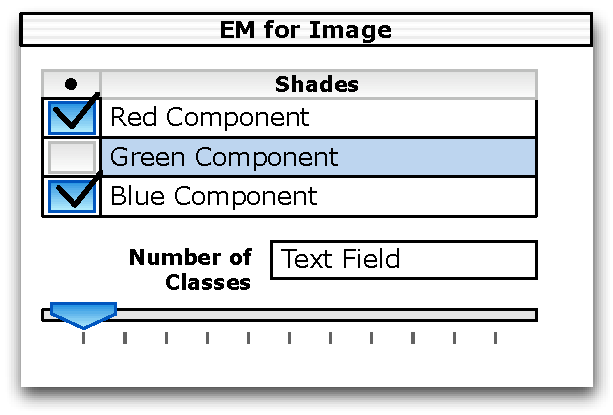
\includegraphics[width=3in]{emComponentSelection.pdf} 
   \caption{The results of an EM for Image
a set of segmenting classifiers, and the 
masks that result from the classification}
   \label{emComponentSelection}
\end{figure}
  


\begin{figure}[htbp] %  figure placement: here, top, bottom, or page
   \centering
   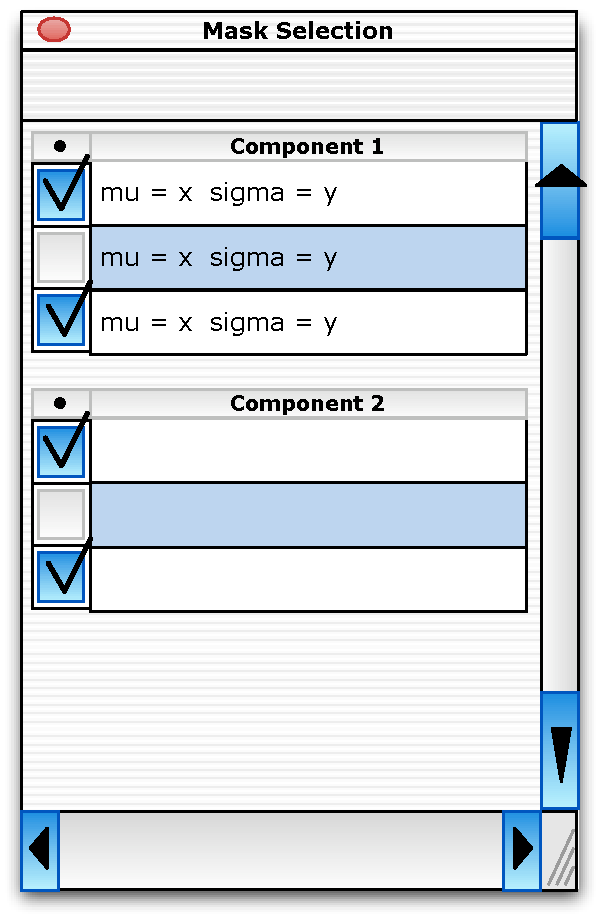
\includegraphics[width=3in]{maskSelector.pdf} 
   \caption{This holds the masks generated by the EM algorithm}
   \label{maskSelector}
\end{figure}

\begin{figure}[htbp] %  figure placement: here, top, bottom, or page
   \centering
   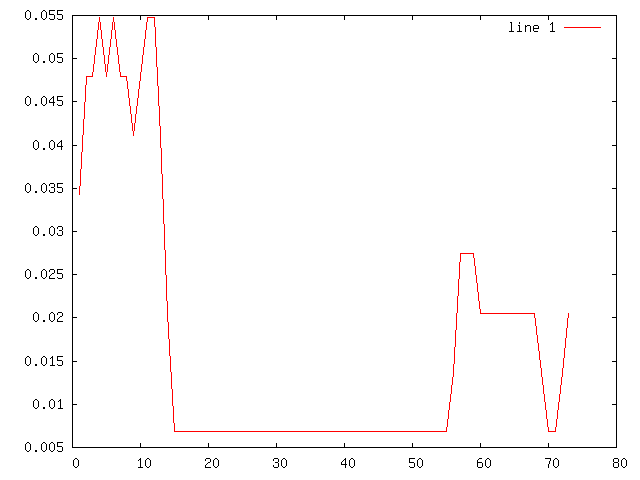
\includegraphics[width=3in]{plot.png} 
   \caption{Plot of Guassians for the Optic Disc}
   \label{histogram-optic-disc}
\end{figure}


\begin{figure}[htbp] %  figure placement: here, top, bottom, or page
   \centering
   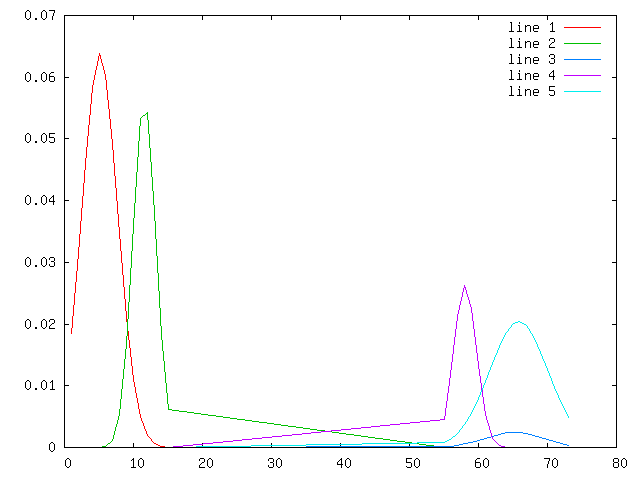
\includegraphics[width=3in]{probability.png} 
   \caption{Plot of sub-Gaussians for the Optic Disc}
   \label{histograms-optic-disc}
\end{figure}

\subsection{Core Graphics Version}
The two steps for EM are explicitly stated in emUnivariateGaussian.  One consequence of this development are revelations about necessary steps for its computation.    The estimation step is computed implicitly first before the loop and again at the end of the loop.  The reason is to compute the estimation termination value.    Another revelation, in listing \ref{lst_maximizationStepEM}, shows the need for careful zeroizing of summing values.  The previous mean is needed in computing the maximization steps variance.    Therefore caution must be applied as to when the mean is computed.  


\begin{lstlisting} [ language={[Objective] C} ,caption={Estimation step of EM, computed explicitly in Objective C}, label=lst_estimationStepEM ] 

-(void) estimationStep
{
	double *mu = [mean localVector];
	double *sigma = [variance localVector];
	double *alpha = [proportions localVector];
	double **A = [mixture localMatrix];
	double *D = [samples localVector];
	
	double amp, sumAlpha = 0;
	Q = 0;
	int r, c; 
	
	for ( r = 0 ; r < numberOfSamples; r++)
		for ( c = 0; c < numberOfClasses; c++)
		{
			amp = alpha[c];
			amp /= sqrt(2 *M_PI * sigma[c]);
			A[r][c] = amp * exp (-0.5 * (D[r] - mu[c])  * (D[r] -mu[c]) / sigma[c]) ;
		}
		
	for ( r = 0 ; r < numberOfSamples; r++)
	{
		sumAlpha = 0;
		for ( c = 0; c < numberOfClasses; c++)
			sumAlpha += A[r][c] ;
		for ( c = 0; c < numberOfClasses; c++)
			A[c][r] /= sumAlpha ;
	}
	
	for ( r = 0; r < numberOfSamples; r++) 
	{
		 sumAlpha = 0.0;
		 for ( c = 0; c < numberOfClasses; c++)
			sumAlpha += A[r][c] ;
		 Q += fabs(log(sumAlpha));
	}
		
	
}

\end{lstlisting}


\begin{lstlisting} [ language={[Objective] C} ,caption={Maximization step of EM, computed explicitly in Objective C}, label=lst_maximizationStepEM ] 

-(void) maximizationStep
{
	double *mu = [mean localVector];
	double *sigma = [variance localVector];
	double *alpha = [proportions localVector];
	double **A = [mixture localMatrix];
	double *Y = [samples localVector];
	
	int r, c; 
	double meanDifference;

	
	[proportions zeroize];
	for ( r =0; r < numberOfSamples; r++) 
		for ( c = 0; c < numberOfClasses; c++)
			alpha[c] += A[r][c];
	
	[variance zeroize];
	for ( r =0; r < numberOfSamples; r++)
		for ( c = 0; c < numberOfClasses; c++)
		{
			meanDifference = Y[r] - mu[c];
			sigma[c]  += A[r][c] * meanDifference * meanDifference;
		}
	for ( c = 0; c < numberOfClasses; c++)
			sigma[c] /= alpha[c];
	
	
	[mean zeroize];
	for ( r =0; r < numberOfSamples; r++)
		for ( c = 0; c < numberOfClasses; c++)
			mu[c]  += A[r][c] * Y[r];
	
	for ( c = 0; c < numberOfClasses; c++)
			mu[c] /= alpha[c];
			
	for ( c = 0; c < numberOfClasses; c++) 
		alpha[c] /= numberOfSamples;

}

\end{lstlisting}

Other components are needed in an Objective-C version to make it more viable, and this is where design decisions must be considered.   In the initial design, obtaining the image data itself was a matter of drawing to a Core Graphics Grey-Scale Bitmap and coping the data out.   This forces the computation to be CPU bound.  Either CPU bound or Graphics Processing Unit bound versions are acceptable.   This subsection illustrates the CPU bound version.   A future report shall review the GPU bound equivalent.  

In order to continue with a DCGMatrix obtained from a Core Graphics Grey-Scale Bitmap, it must be transformed into a vector of equal number of elements.  This vector and the number of desired classifications must then initialize an emUnivariateGaussian.    Once initialized, it is convenient to extract the results into an NSArray containing the sufficient statistics.  Such an array need not retain the proportions value.  

Once obtain the array of sufficient statistics becomes the classifier for every grey scale value in the image.  In this case, the user is allowed to select which classifiers he/she wishes to see.   It is the point of selecting classifiers that a mask is drawn.  A mask has the sole purpose of blending sections of the image.   In this case, either the color point belongs or it does not.     It is here that Core Graphics Data Providers and Image Providers become useful.   Also, it is here where the DCGMatrix obtained from the Grey-Scale Bitmap is reused, and fed into the classifier.  If the point belongs, a white value is inserted into the mask.  The mask is black otherwise.   Note that a true color filter would have use a multivariate variety of the classifier as it is a vector (color vector).    

It should be noted that obtaining the DCGMatrix from the Core Graphics Grey Scale Bitmap is quite tricky.  It is one section that is anything, but universal between PPC and x86 architectures.   Care has to be taken to ensure byte ordering on the bitmap.  Otherwise, the results are garbage, and the EM will compute nonsense.  

The first successful version used a subclass of NSOpenGLView and model controller to test the concept of an EM filter.  A better version should move the computation to a CIFilter, and use threads to move the computation away from the main display thread.   Otherwise, the intensity of computation can overwhelm the main thread, and waste the existence of multiple-core CPUs and computational grids.   With the first version, the control includes a panel to show the segments (displayed by mean and variance show in figure \ref{segmentsPanel} ) and view window that shows the image masked with the selected segment.  If no segment is selected, the mask is clear and shows the original image, shown in figure \ref{fiveEmSegments}.  

\begin{figure}[htbp] %  figure placement: here, top, bottom, or page
   \centering
   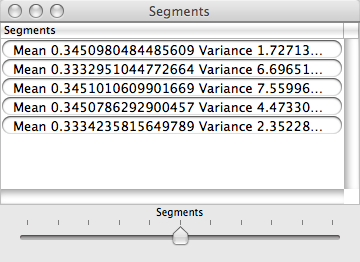
\includegraphics[width=3in]{segmentsPanel.png} 
   \caption{EM Segments shown by mean and variance for a photo of a human iris.}
   \label{segmentsPanel}
\end{figure}

\begin{figure}[htbp] %  figure placement: here, top, bottom, or page
   \centering
   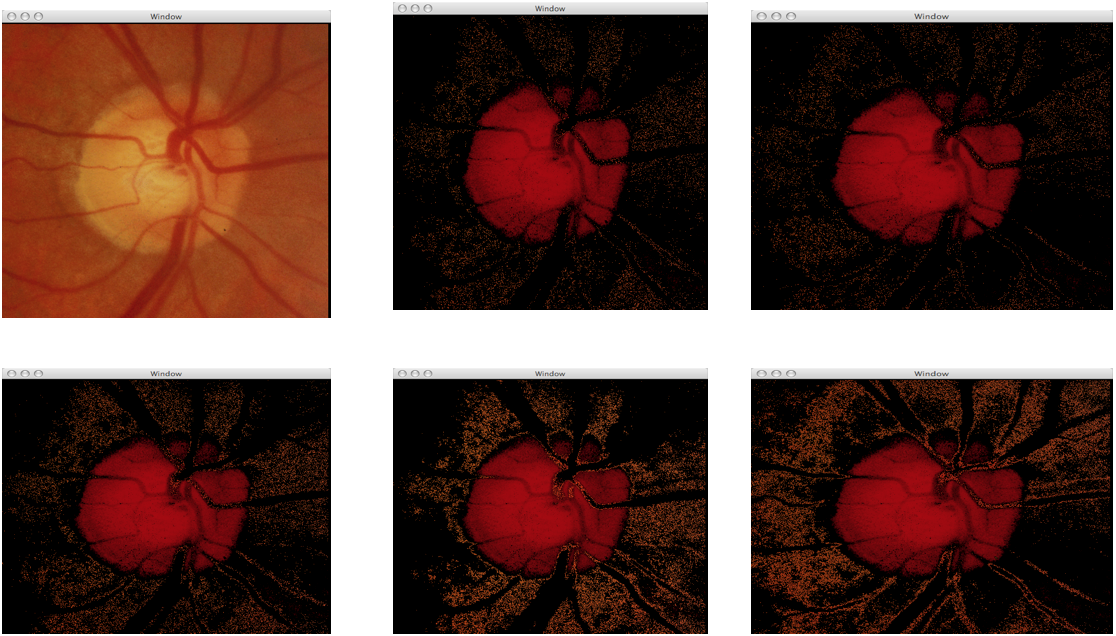
\includegraphics[width=6in]{fiveEmSegments.png} 
   \caption{Both the original image and 5 EM Segments of a human iris. }
   \label{fiveEmSegments}
\end{figure}

There is the possibility of computing the EM directly from the Graphics Card, but that implies providing an expected step kernel, a maximization step kernel,  termination test kernel.  

\bibliography{../../patternNotes.bib}
\bibliographystyle{abbrv}
\end{document}  